\documentclass[9pt]{IEEEtran}

\usepackage[english]{babel}
\usepackage{graphicx}
\usepackage{epstopdf}
\usepackage{fancyhdr}
\usepackage{amsmath}
\usepackage{amsthm}
\usepackage{amssymb}
\usepackage{url}
\usepackage{array}
\usepackage{textcomp}
\usepackage{listings}
\usepackage{hyperref}
\usepackage{xcolor}
\usepackage{colortbl}
\usepackage{float}
\usepackage{gensymb}
\usepackage{longtable}
\usepackage{supertabular}
\usepackage{multicol}

\usepackage[utf8x]{inputenc}

\usepackage[T1]{fontenc}
\usepackage{lmodern}
\input{glyphtounicode}
\pdfgentounicode=1

\graphicspath{{./figures/}}
\DeclareGraphicsExtensions{.pdf,.png,.jpg,.eps}

% correct bad hyphenation here
\hyphenation{op-tical net-works semi-conduc-tor trig-gs}

% ============================================================================================

\title{\vspace{0ex}
Project Title}

\author{Firs-name Last-name\vspace{-4.0ex}}

% ============================================================================================

\begin{document}

\maketitle

\section{Introduction}

A brief description of the problem and how you have solved it. This should be a short paragraph - just a few sentences is enough.
Do not repeat text from instructions, but rather briefly summarize what is the main problem.
Note that the page limit is two pages, so make sure that you write only that is the most important.

\section{Experiments}

This section should be structured so that it answers the questions/tasks given at the end of the instructions document (Section Grading). 
Make sure that each experiment is supported with a figure or table and do not forget to reference it in text (e.g., see Figure~\ref{fig:figure_label}). 
Figures which are included in the report should be as compact as possible due to the page limit.
Result of each experiment should be described in text. When describing performance of some method or some figure - do not write what is obvious, but rather try to find reasons for such behaviour.

Example: 
{\it In Figure~\ref{fig:figure_label} (bottom-right) if a field of optical flow, which is small near the center and large at the edges of the image.}
This is a bad description of the result since it is obvious from the image that the arrows around the center are short and long at the edges.
A better description could be:
{\it The optical flow field in Figure~\ref{fig:figure_label} (bottom-right) is small near the center and large at the edges of the image since pixels near the edges move much more than center pixels during rotation.}

An important part of the report is analysis of the failure cases. 
Show failure cases, discuss the reasons for them and try to say how would you improve the performance in these cases.

\begin{figure}[h]
    \centering
    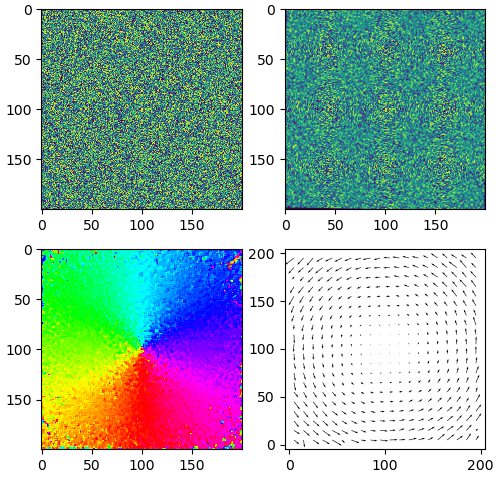
\includegraphics[width=1\columnwidth]{figure.png}
    \caption{Figure caption.}
    \label{fig:figure_label}
\end{figure}


\section{Conclusion}

A sentence or two to conclude the report. Write when the method works well and what its limitations.

\bibliographystyle{IEEEtran}
\bibliography{bibliography}

\end{document}
